\documentclass[10pt,a4paper,titlepage]{article}
\usepackage[utf8]{inputenc}
\usepackage{amsmath}
\usepackage{amsfonts}
\usepackage{amssymb}
\usepackage{graphicx}
\author{Claude Goubet}
\title{Getting Familiar With Synchrotron-CT Data}
\begin{document}
\maketitle


\section{Data Characteristics}
\begin{itemize}
	\item number of projections:
	\item resolution:
	\item number of angles:
	\item Rotation axis
	\item ...
	
\end{itemize}

\section{Reading The Data}
	\subsection{Projections}
		show 4 different projection out of 100
	\subsection{Sinogram}
		show 4 sinograms over different slices\\
		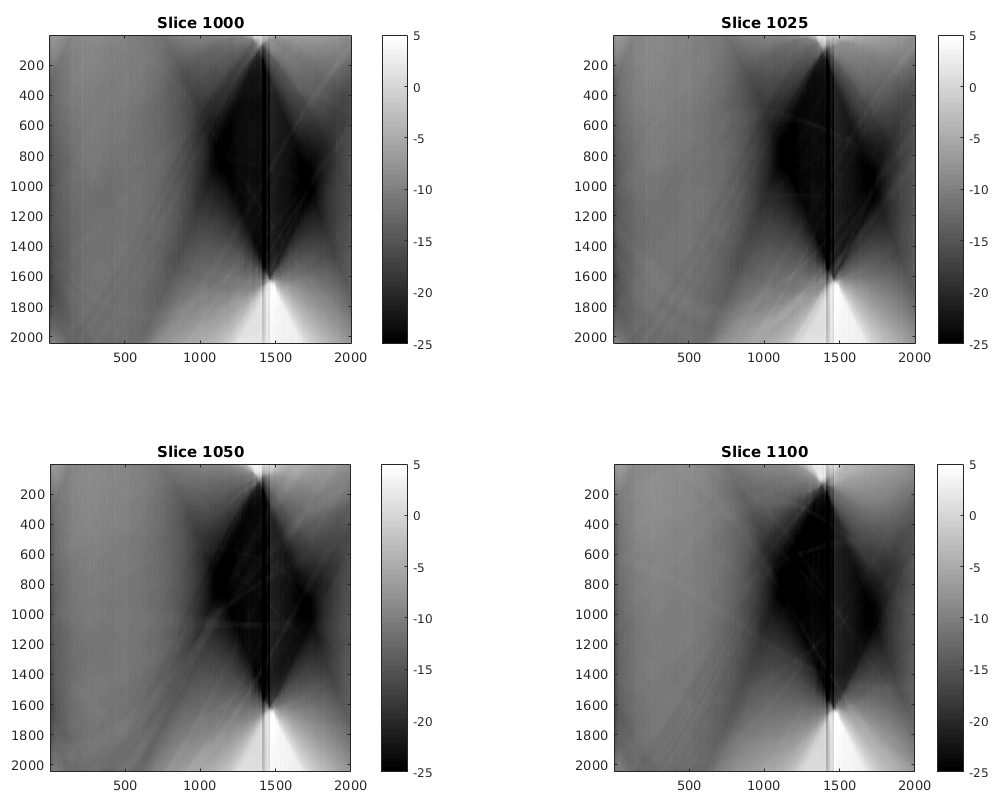
\includegraphics[width=\textwidth]{sinograms/Sinograms2.png}	
		for individual images refer to index section \ref{SinoImg}

	
\section{FBP Reconstruction}
	\subsection{Reconstruction without zero-padding default filter}
		Show 4 different reconstructed images
	\subsection{Reconstruction with zero-padding}
		\subsubsection{Using matlab default filter}
			Show 4 different reconstructed images
		\subsubsection{Comparing frequency scaling (?) one slice}
			try with 0.7 0.4 0.6...
		\subsubsection{Comparing matlab Filters}
			try all filters proposed for iradon
	\subsection{Reduced number of projections}
		show 2000, 1000, 700, 400, 200, 100 projections\\
		show difference between ref (2000)
		
\section{iterative reconstruction}	

\section{Index}
	\subsection{Sinogram}
		\label{SinoImg}
		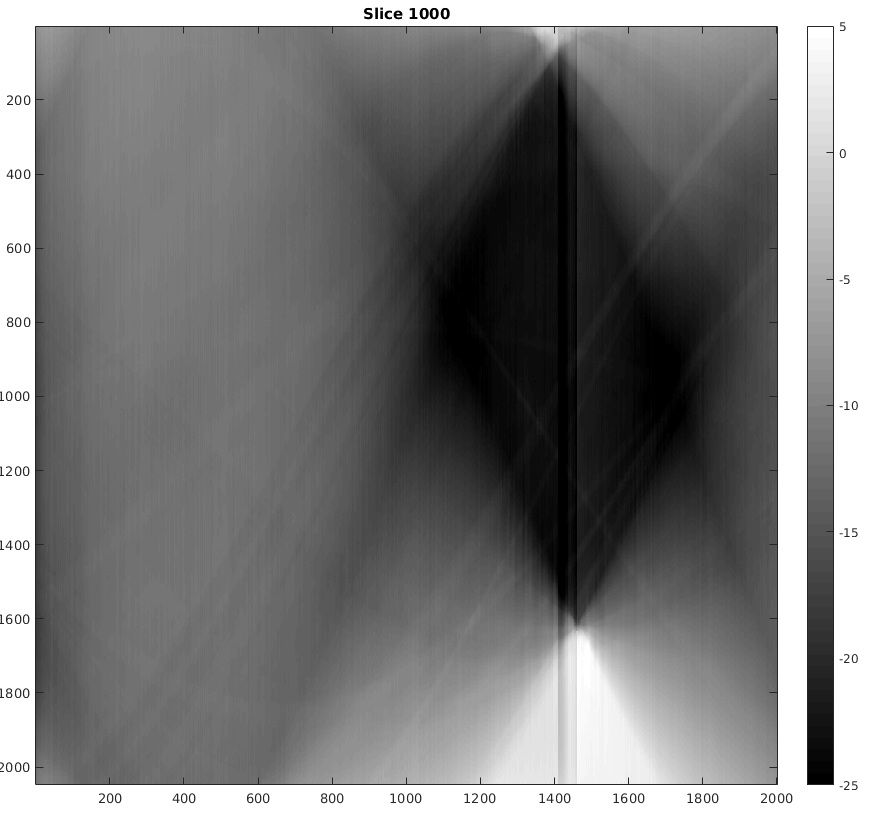
\includegraphics[width=\textwidth]{sinograms/Slice1000.png}
		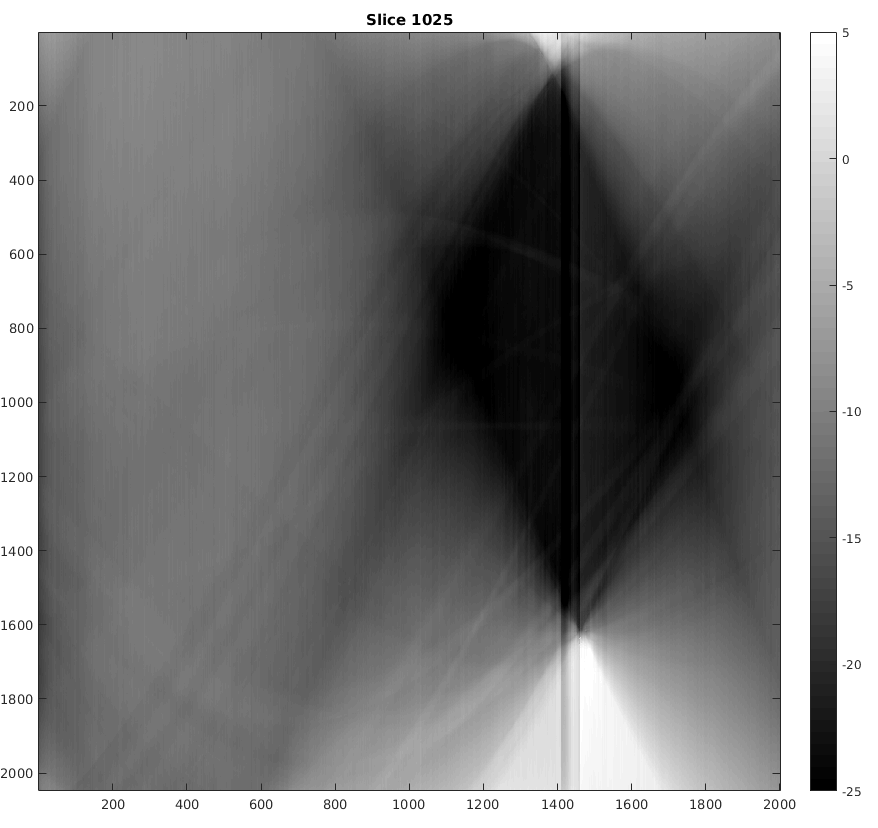
\includegraphics[width=\textwidth]{sinograms/Slice1025.png}
		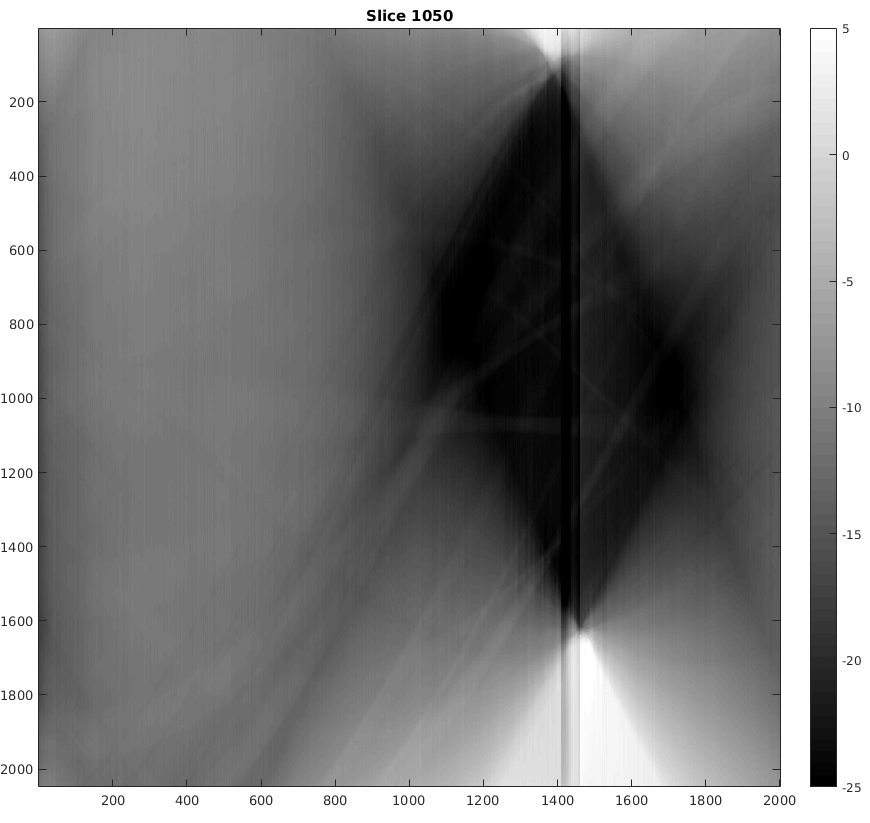
\includegraphics[width=\textwidth]{sinograms/Slice1050.png}
		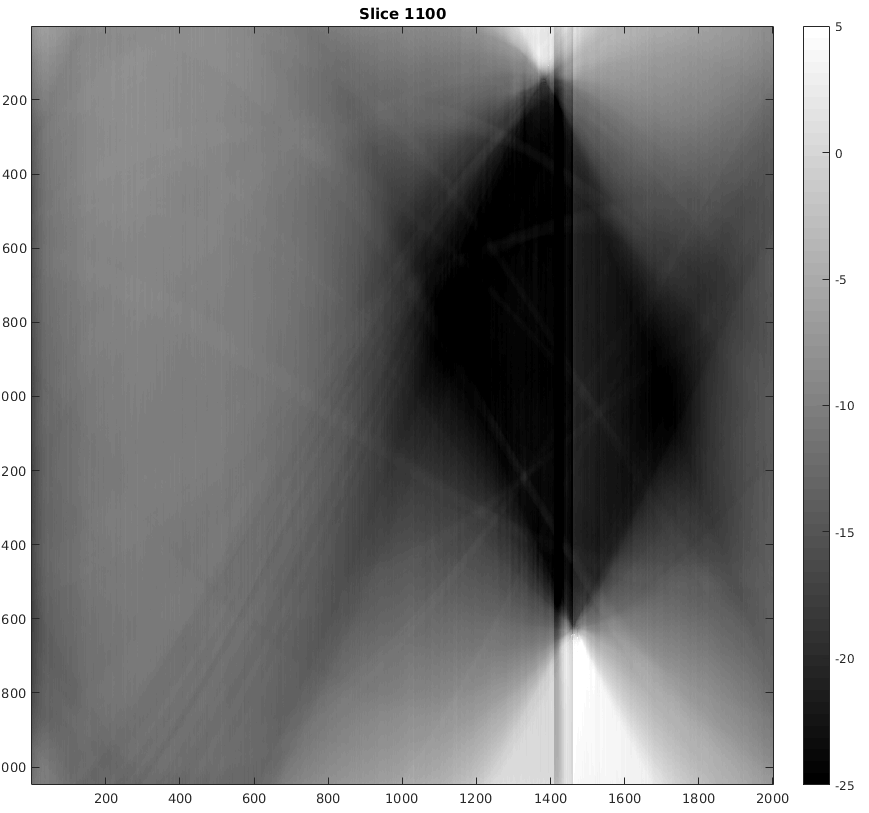
\includegraphics[width=\textwidth]{sinograms/Slice1100.png}

\end{document}